\subsubsection{HL-LHC projections of LHCb searches for 2HDM+S pseudoscalars}
\begin{center}
 Martino~Borsato$^{1}$, Ulrich~Haisch$^{2,3,4}$, Jernej~F.~Kamenik$^{5,6}$, \\ Augustinas~Malinauskas$^3$, and Michael Spira$^{7}$\\
 \vspace{3mm}
\centerline{{\it $^{1}$Physikalisches Institut, Ruprecht-Karls-Universit\"{a}t Heidelberg, Heidelberg, Germany}}
\centerline{{\it  $^{2}$Max Planck Institute for Physics, F{\"o}hringer Ring 6, 80805 M{\"u}nchen, Germany}}
\centerline{{\it  $^{3}$Rudolf Peierls Centre for Theoretical Physics, University of Oxford, OX1 3NP Oxford, United Kingdom}}
\centerline{{\it  $^{4}$CERN, Theoretical Physics Department, CH-1211 Geneva 23, Switzerland}}
\centerline{{\it  $^{5}$Jo\v{z}ef Stefan Institute, Jamova 39, 1000 Ljubljana, Slovenia}}
\centerline{{\it  $^{6}$Faculty of Mathematics and Physics, University of Ljubljana, Jadranska 19, 1000 Ljubljana, Slovenia}}
\centerline{{\it  $^{7}$Paul Scherrer Institut, CH-5232 Villigen PSI, Switzerland}}
\end{center}

Several well-motivated extensions of the Standard Model~(SM) include a new pseudoscalar $a$ with mass below the electroweak scale. A well-known example in the context of supersymmetry is the next-to-minimal supersymmetric SM, where this state can arise as a result of an approximate global $U(1)_R$ symmetry~\cite{Dobrescu:2000yn}. Non-supersymmetric extensions featuring a light pseudoscalar include Little Higgs models, hidden valley scenarios (see~\cite{Curtin:2013fra}, and references therein for details), and simplified models where a complex singlet scalar is coupled to the Higgs potential of the SM or the two-Higgs doublet model~(2HDM). Light pseudoscalars have been searched via various collider signatures such as exotic decays of the $125 \, {\rm GeV}$ scalar $h$ discovered at the LHC (both $h\to aa$ and $h\to aZ$), radiative decays of bottomonium $\Upsilon\to a\gamma$, direct production from $pp$ collisions in association with $b$-jets and also inclusively in $pp\to a+X$, where the main production mode is usually gluon-gluon fusion. The interplay of searches for exotic $h$ decays and direct searches in $pp$ collisions within 2HDM+S models depend on the 2HDM parameters $\alpha, \beta$, on the mixing angle $\theta$, on the physical spin-0 masses, and on the form of the scalar potential (see for instance~\cite{Haisch:2018kqx} for further explanations).

Despite the significantly lower luminosity collected with respect to ATLAS and CMS, LHCb has proven to be capable of placing world-best limits for low-mass pseudoscalars produced in gluon-gluon fusion~\cite{Haisch:2016hzu,Haisch:2018kqx}, by searching simply for resonant pairs of opposite-sign muons~\cite{Aaij:2017rft, Aaij:2018xpt}. Indeed, a large fraction of these light pseudoscalars are produced with large boosts at the LHC and end up in the LHCb acceptance. On top of that, the LHCb detector is capable of triggering on muons with transverse momenta as low as $1.8 \, {\rm GeV}$ ($0.5 \, {\rm GeV}$) with the current (upgraded) trigger, greatly enhancing its acceptance to $a\to\mu^+\mu^-$ with respect to ATLAS and CMS. A key ingredient of this trigger, is the LHCb capability to efficiently reject  the large background due to pion mis-identification thanks to online availability of offline-quality particle identification based on information from all sub-detectors~\cite{Aaij:2016rxn, Dujany:2015lxd}. On top of that, the large boost of the pseudoscalar $a$  in the forward region allows to separate muons coming from semileptonic $B$ decays due to their displacement with respect to the $pp$ collision vertex. 

The HL-LHC sensitivity to prompt dimuon resonances in the context of dark photon searches at LHCb can be found in~\cite{Bediaga:2018lhg}. The kinematic selection used for the projection is inspired by~\cite{Ilten:2016tkc} and rely on the improved performance expected after the upgrade of the LHCb trigger that will be implemented for LHC Run-3. Maintaining this exceptional performance in the HL-LHC era (\ie with 10 times larger instantaneous luminosity) will require a redesign of the muon detector and is briefly discussed in~\cite{Bediaga:2018lhg}.

\begin{figure}[ht!]
\centering
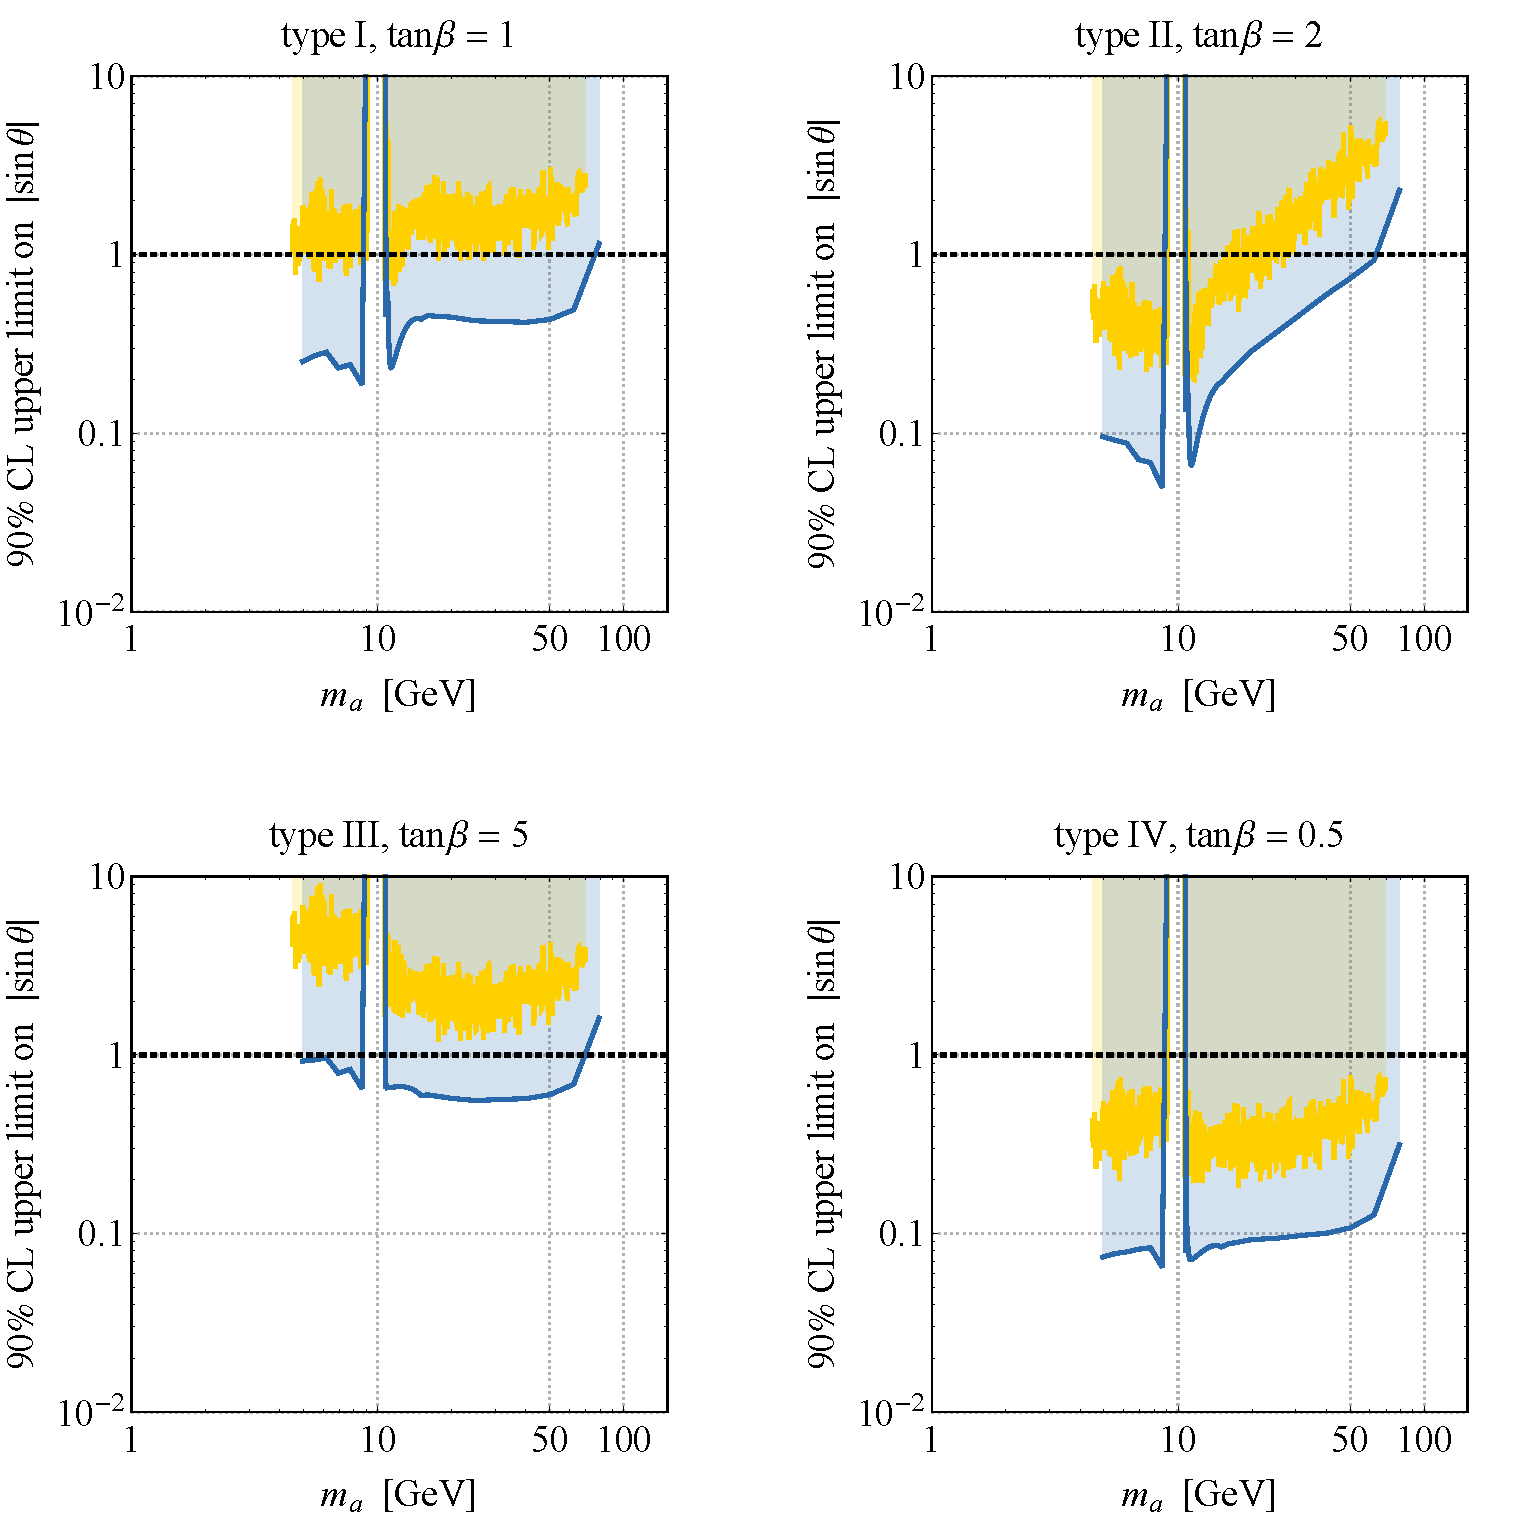
\includegraphics[width=\textwidth]{\main/section9/plots/LHCbprojections.pdf}
\vspace{2mm}
\caption{Upper $90\%$ CL limits on $|\!\sin\theta|$ in the 2HDM+S of type~I with $\tan\beta =1$ (top left), type~II with $\tan\beta =2$ (top right), type~III with $\tan\beta = 5$ (bottom left) and type~IV with $\tan\beta = 0.5$ (bottom right). The yellow curves illustrate the results of a recast~\cite{Haisch:2018kqx} of the LHCb search~\cite{Aaij:2017rft} performed with a data set corresponding to $1.6\, {\rm fb}^{-1}$ of $13 \, {\rm TeV}$ $pp$ collisions, while the blue contours are our projections to $300 \, {\rm fb}^{-1}$ of $14 \, {\rm TeV}$ $pp$ collision data using the expected HL-LHC dark photon limits presented in~\cite{Bediaga:2018lhg}. }\label{fig:lhcb_lightmumu}
\end{figure}

In Figure~\ref{fig:lhcb_lightmumu}, the limits on the dark photon parameter space presented in~\cite{Bediaga:2018lhg} are reinterpreted in the context of the 2HDM+S, following the analysis strategy detailed in~\cite{Haisch:2018kqx}. The production cross section of the pseudoscalar $a$ and its decay rate to muons depend on the mixing angle $\theta$, on the parameter $\tan\beta$ and on the type of the Yukawa sector of the considered 2HDM. Fixing $\tan\beta$ and the type of the 2HDM, upper limits are placed on $|\!\sin\theta|$ as a function of the pseudoscalar mass $m_a$. In all considered cases, LHCb searches in the HL-LHC era~(blue contours) are found to be sensitive to values of $|\!\sin\theta|$ well below 1 for a large range of~$m_a$ values between $5 \, {\rm GeV}$ and $70 \, {\rm GeV}$. This represents a significant improvement over the LHC Run-2 results~(yellow curves), where only in the 2HDM+S scenario of type IV with $\tan \beta = 0.5$ it was possible to set physical meaningful bounds on the sine of the mixing angle $\theta$, \ie $|\!\sin\theta| < 1$, in the entire range of considered pseudoscalar masses. Notice that spin-0 states with masses around $10 \, {\rm GeV}$ can be probed by searches for dimuon resonances in $\Upsilon$ production~\cite{Haisch:2016hzu,Aaij:2018xpt}.
